\documentclass{article}
\usepackage[T1]{fontenc}
\usepackage{lmodern}
\usepackage{graphicx}
\usepackage{amsmath,amssymb}
\usepackage[a4paper,margin=2cm]{geometry}
\usepackage[absolute,overlay]{textpos}
\setlength{\TPHorizModule}{1mm}
\setlength{\TPVertModule}{1mm}
\usepackage[indonesian]{babel}
\usepackage{hyperref}
\setlength{\emergencystretch}{2em}
% unit: Halaman 67

\begin{document}

% === Halaman 67 (llm) ===

\vspace{160.38mm}

Contoh jaringan Feistel di dalam DES:\
\vspace{60mm}
Jaringan $Feistel$ pada enkripsi putaran ke-$i$
\[ 
\begin{aligned}
L_i &= R_{i-1} \\
R_i &= L_{i-1} \oplus f(R_{i-1}, K_i)
\end{aligned}
\]

% deskripsi: Diagram alir jaringan Feistel yang menunjukkan proses transformasi data antara L dan R menggunakan fungsi f dan kunci Ki.
% bbox normalisasi: [0.1400, 0.2300, 0.8200, 0.7700]
\begin{textblock*}{142.80mm}(29.40mm,68.31mm)
\noindent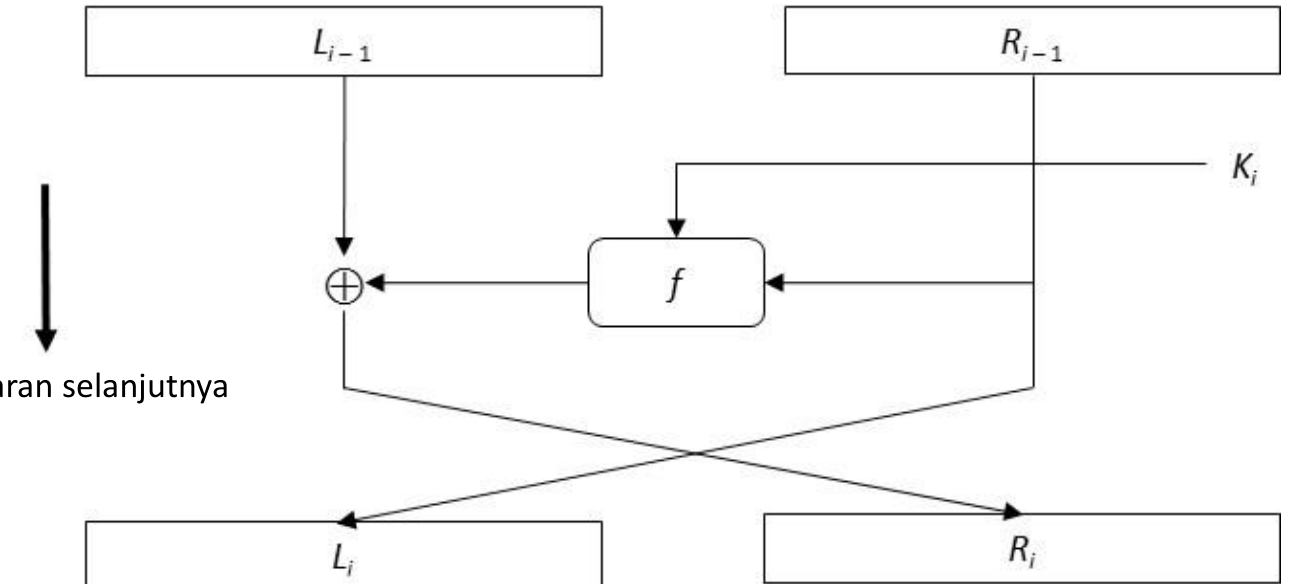
\includegraphics[width=142.80mm,height=160.38mm]{../../images/llm/page_067_img_01.png}%
\end{textblock*}

\end{document}
